\documentclass[12pt]{article}
\usepackage{preamble}
\graphicspath{{pics/ps1a/}}
\begin{document}
% \maketitle
\lhead{Problem Set 1a}

%%%%%%%%%%%%%%%%%%%%%%%%%%%%%%%%%%%%%%%%%%%%%%%
%                  Definitions                %
%%%%%%%%%%%%%%%%%%%%%%%%%%%%%%%%%%%%%%%%%%%%%%%
%\includegraphics[width=\mywidth\textwidth]{}

% \begin{figure}[h!]
% \centering
% \input{pics/PS2/p7b}
% \caption{}
% \label{fig-}
% \end{figure}

% \begin{enumerate}[label=\alph*.]
%     \setcounter{enumi}{1}
%     \item 
% \end{enumerate}
\renewcommand{\vem}{\newpage}


%%%%%%%%%%%%%%%%%%%%%%%%%%%%%%%%%%%%%%%%%%%%%%%
%                Problem 1                    %
%%%%%%%%%%%%%%%%%%%%%%%%%%%%%%%%%%%%%%%%%%%%%%%
\problem{1.*Let it Snow!}{
Before getting started with the data work, first consider the table from Snow (1855)
reproduced in the lecture notes (“Snow’s Table IX”). The table reports only means.
\begin{enumerate}[label=(\alph*)]
    \item Develop an approximate 95\% confidence interval for ``Deaths per 10,000 Houses'' for Southwark and Vaxhall customers. Develop another 95\% CI for the same quantity for Lambeth. Do the confidence intervals overlap?
    \end{enumerate} 
}

\begin{figure}[ht!]
\centering
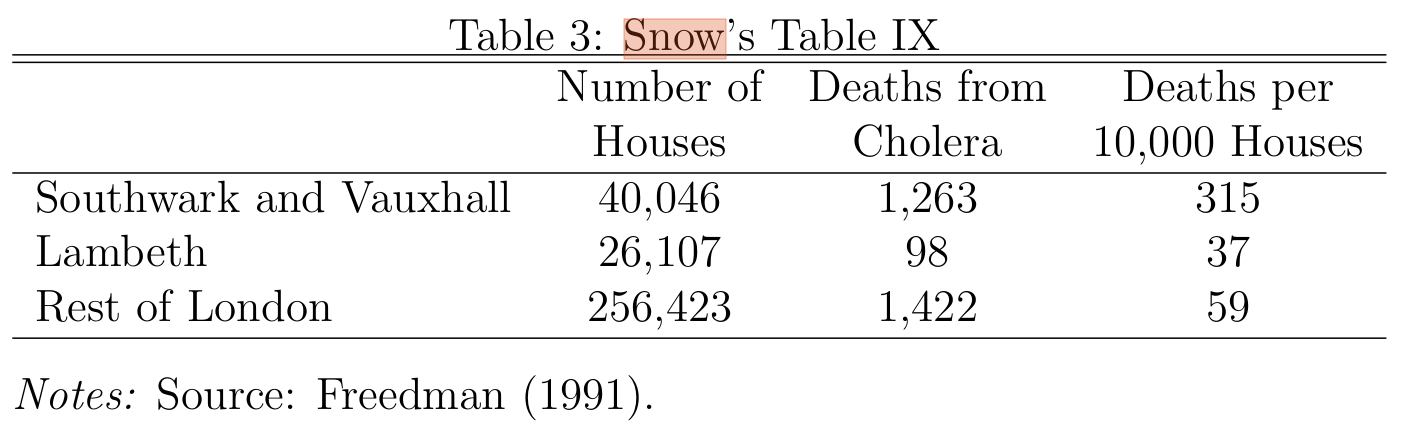
\includegraphics[width=0.8\textwidth]{snow_table}
\caption{The orginal table from \textit{On the Mode of Communication of Cholera} (John Snow, 1855). Note the rate of deaths per 10,000 houses for the Rest of London is incorrect based on the first two columns. $\sfrac{1,422}{256,423}\cdot 10,000\approx 55.5$ not 59.}
\label{fig-1}
\end{figure}

\begin{align*}
\intertext{Assuming that, within a region $k\in\{a, b, c\}$, the indicator of one person in household $i$ dying from Cholera $X^k_i$ is distributed as a Bernoulli random variable with probability $p_k$ -- $X^k_i\iid \text{Bernoulli}(p_k)$. Then deaths per 10,000 households in region $k$, $R_k$, is a function of the sum of i.i.d. Bernoulli random variables. Let $N_k$ be the number of houses in region $k$, then}
R_k &= \frac{10,000}{N_k}\sum\limits_{i=1}^{N_k}X^k_i 
    \sim  \frac{10,000}{N_k}\text{Binom}(N_k, p_k)
\intertext{Let $Z^k\sim\text{Binom}(N_k, p_k)$. Then the variance of $R_k$ is}
\text{var}(R_k) &= \text{var}(\frac{10,000}{N_k}Z^k) \\
    &= \left(\frac{10,000}{N_k}\right)^2\text{var}(Z^k) \\
    &= \left(\frac{10,000}{N_k}\right)^2 N_k\cdot p_k\cdot (1-p_k) \\
    &= \frac{(10,000)^2}{N_k} p_k(1-p_k) \\
\intertext{Let $ z_{\alpha}$ be the z-score at significance level $\alpha$. Then, for large enough $N_k$ (which 26,000 is probably large enough), the 95\% ($\alpha = (1-95\%)/2$) confidence interval for $R_k$ would be:}
\text{CI}_{95} &= R_k \pm z_\alpha\sqrt{\text{var}(R_k)} \\
    &= R_k \pm z_\alpha\sqrt{\frac{(10,000)^2}{N_k} p_k(1-p_k) } \\
    &= R_k \pm 10,000z_\alpha\sqrt{\frac{p_k(1-p_k)}{N_k}} \\
\intertext{And an unbiased estimator for the probability of death $p_k$ would be the mean of the indicators:}
\hat{p}_k &= \frac{1}{N_k}\sum\limits_{i=1}^{N_k}X^k_i 
    = \frac{D_k}{N_k}
    = \overline{X^k_i}
\shortintertext{where $D_k$ is the number of deaths in region $k$ (the sum of the $X^k_i$'s).}
\end{align*}

Calculating $\hat{p}_k$ from the Snow table, we get

% Table generated from ps1a.R in github repo
\begin{table}[h!]
\centering
\begin{tabular}{cccc}
  \hline
$k$ & $R_k$  & CI$_k$ lower  & CI$_k$ upper \\ 
  \hline
a & 315.39 & 298.27 & 332.50 \\ 
b & 37.54 & 30.12 & 44.96 \\ 
c & 55.46 & 52.58 & 58.33 \\ 
   \hline
   \hline
\end{tabular}
\end{table}

No, the confidence intervals for regions $a$ and $b$ do not overlap.


%%%%%%%%%%%%%%%%%
%     Part b    %
%%%%%%%%%%%%%%%%%
\vem
\problem{}{
    \begin{enumerate}[label=(\alph*)]
    \setcounter{enumi}{1}
    \item Discuss either formally or intuitively the critical assumption that underlies your confidence intervals. Give a 2 or 3 sentence quote from Snow’s description (re-produced in Freedman (1991)) that supports this assumption.
    \end{enumerate} 
}

The critical assumption of the above calculation is the the observations in each of the regions $k$ are statistically independent of each other -- that the probability of death in one region is not affected by the probability or realization of death in the other region, or by the underlying characteristics of the population in the different regions. Because the different regions were being supplied from different water sources, then conditional on the upstream water supply not being contaminated, if we assume the water water was the source of Cholera infection, then the two groups death rates should be independent. 

To support this idea, this section, from pg 75, of Snow's 1955 book is of interest:

\begin{displayquote}
Each Company supplies both rich and poor, both large houses and small; there is no difference either in the condition or occupation of the persons receiving the water of the different Companies\dots\\[-1em]

\dots The experiment, too, was on the grandest scale. No fewer than three hundred thousand people of both sexes, of every age and occupation, and of every rank and station, from gentlefolks down to the very poor, were divided into two groups without their choice, and, in most cases, without their knowledge; one group being supplied with water containing the sewage of London, and, amongst it,  whatever might have come from the cholera patients, the other group having water quite free from such impurity.
\end{displayquote}

This natural experiment provided evidence that, even when the groups are essentially identical in distributions of characteristics and treatment of water supply is as good as random, that the group getting the water from downstream was statistically significantly more likely to die from Cholera.



%%%%%%%%%%%%%%%%%
%     Part c    %
%%%%%%%%%%%%%%%%%
\vem
\problem{}{
We now move to some analysis of real data. The data portions of Problem Sets 1a and
1b are based heavily on the paper Almond, Chay, and Lee (2005), and problem sets from
Ken Chay and John DiNardo based on some of the data used in the paper. The goal of
this assignment is to examine the research question: what is the causal effect of maternal
smoking during pregnancy on infant birthweight and other infant health outcomes. The
data for the problem set is an extract of all births from the 1993 National Natality Detail
Files for Pennsylvania. Each observation represents an infant-mother match. The data in
Stata format can be downloaded from the bCourses website. There should be 48 variables
in the data and, after you are finished with the cleaning steps described below, 114,610
observations.\\

The data here are “real” and quite imperfect, which will help simulate the unpleasantness
of real world data work. Unlike the real world where you will confront this bleak situation
largely alone, I will provide you with some hints for working your way through the raw data.
You can download part of the codebook for the data to help you figure out the relevant
variables.
}



\newpage
%%%%%%%%%%%%%%%%%%%%%%%%%%%%%%%%%%%%%%%%%%%%%%%
%                Problem II                   %
%%%%%%%%%%%%%%%%%%%%%%%%%%%%%%%%%%%%%%%%%%%%%%%
\problem{2. Real Data}{
The first order of business is to go through the code book, decide on the relevant
variables, and process the data. This involves several steps: \\
    \begin{enumerate}[label=(\alph*)]
        \item Fix missing values. In the the data set several variables take on a value of, say, 9999 if missing. We have already checked for missing observations for about 2/3 of the variables. The remaining variables need to be checked and are the last 15 in the variable list (i.e. from ’cardiac’ to ’wgain’). Refer to the codebook for missing value codes. Produce an analysis data set that drops any observation with missing values.
    \end{enumerate} 
}

% table generated from code in ps1a.R in github repo
\begin{table}[ht]
\centering
\caption{Missing values, by variable name.} 
\begin{tabular}{lrr}
  \hline
varname & missing\_code & num\_missing \\ 
  \hline
herpes &   8 &   6 \\ 
  tobacco &   9 &  65 \\ 
  cigar &  99 & 1077 \\ 
  cigar6 &   6 & 1077 \\ 
  alcohol &   9 & 105 \\ 
  drink &  99 & 2116 \\ 
  drink5 &   5 & 2116 \\ 
  wgain &  99 & 3048 \\ 
   \hline
\end{tabular}
\end{table}

The observations with missing values have been removed, bringing our number of observations down from 120,461 to 114,610 (5851 observations dropped).

%%%%%%%%%%%%%%%%%
%     Part b   %
%%%%%%%%%%%%%%%%%
\vem
\problem{}{
    \begin{enumerate}[label=(\alph*)]
    \setcounter{enumi}{1}
        \item If this were a real research project you would want to consider other approaches to missing data besides termination with extreme prejudice. What observations do you have to drop because of missing data. Might this affect your results? Do the data appear to be missing completely at random? How might you assess whether the data appear to be missing at random?
    \end{enumerate} 
}

The data do not appear to be missing completely at random. MCAR (Missing Completely at Random) implies that there is no relationship between the missing observations and the observable variables, but we can see from figure \ref{fig-2b1} that the distribution of cigarette smoking is different between observations that have missing drink and those that are not missing drink. We also see that most observations missing tobacco are also missing drink.

Another crude method to see this is to create a single dummy variable for missingness in any variable. Then, using the dummy to create two sub-samples, one which has complete data, and another with any missingness, we can conduct a series of t-tests (with 5\% signficance level) on whether means of each variables are different across the two sub-samples. We reject null of equivalence on 37 out of 48 variables, giving another evidence that missing is not completely random.

We could further explore missing relationships by running regressions of the variables on the missingingness indicators for several other variables, then testing if the coefficient on the indicators is significantly different from zero. We would need to be a bit more precise, but this could produce a test of significance of a relationship with the other variables. This would at least test for MCAR. 

The problem with testing MAR is that the assumption is violated when missingness depends on unobservables. This is inherently hard to test.

\begin{figure}[!ht]
\centering
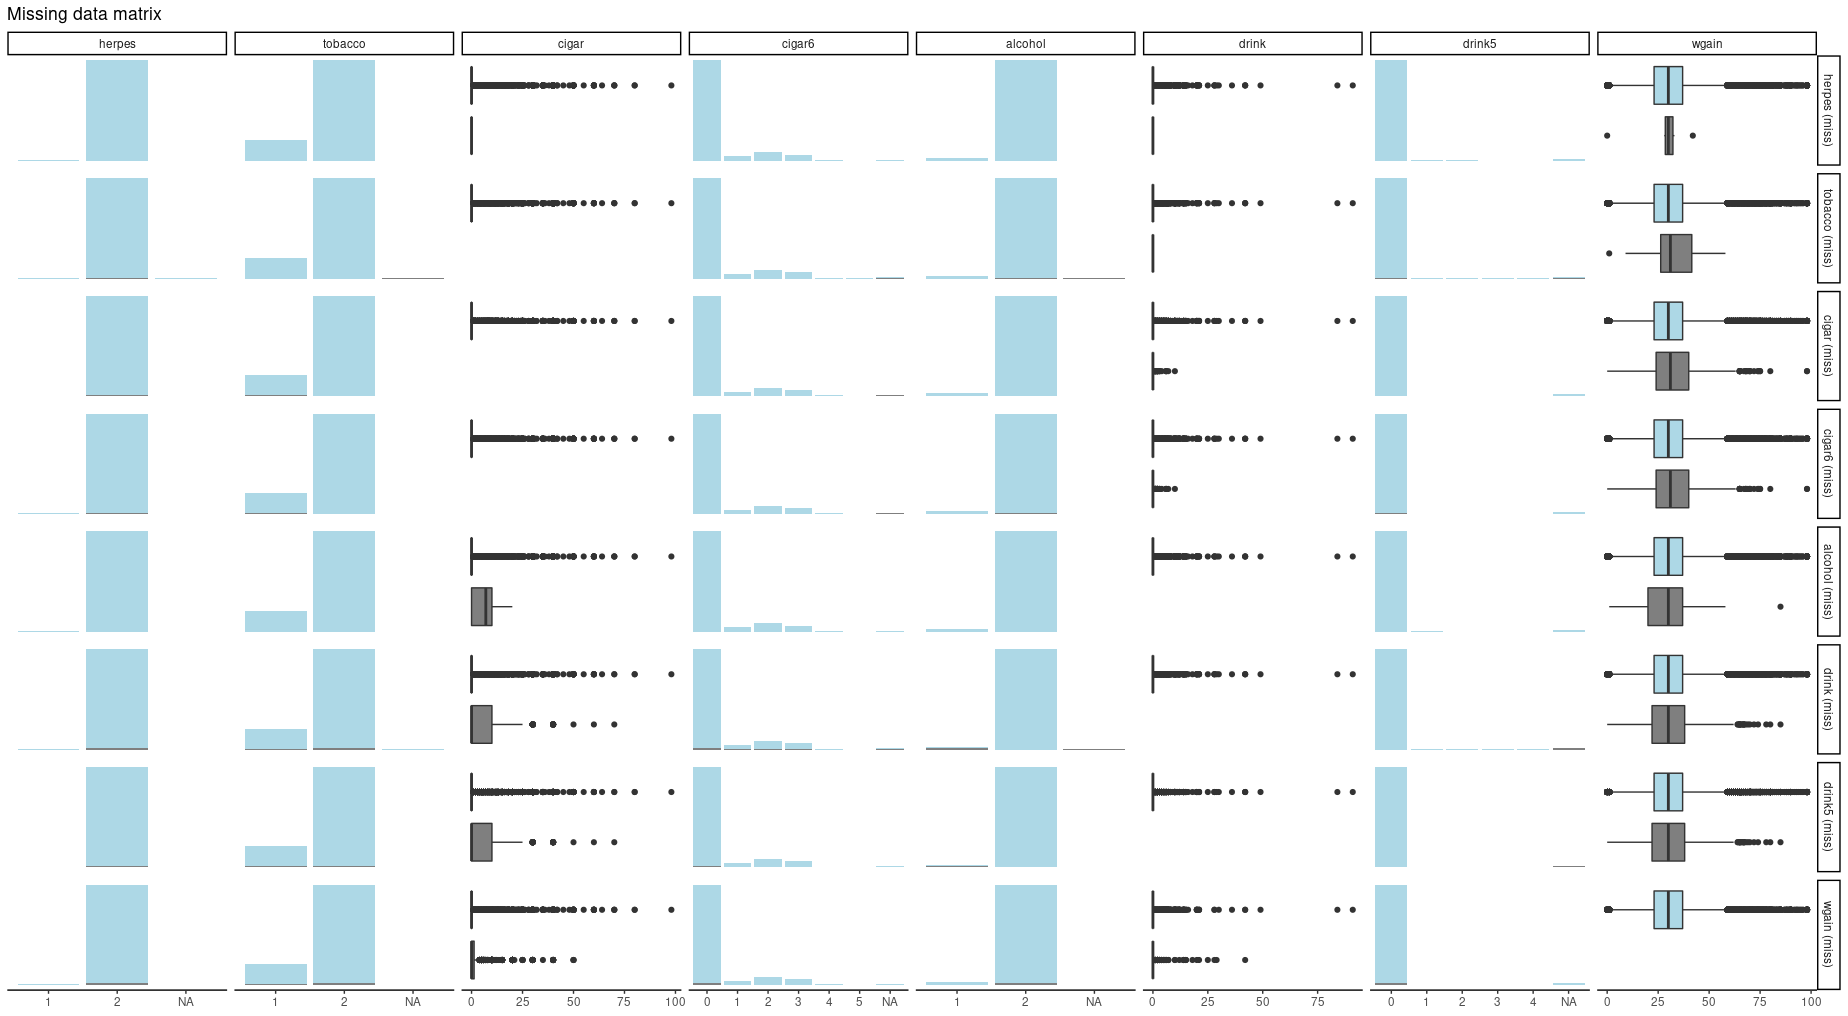
\includegraphics[width=\textwidth]{2b-missing_plots.png}
\caption{A plot to show the distribution of variables, broken out by missing and not missing in other variables.}
\label{fig-2b1}
\end{figure}

\begin{figure}[!ht]
\centering
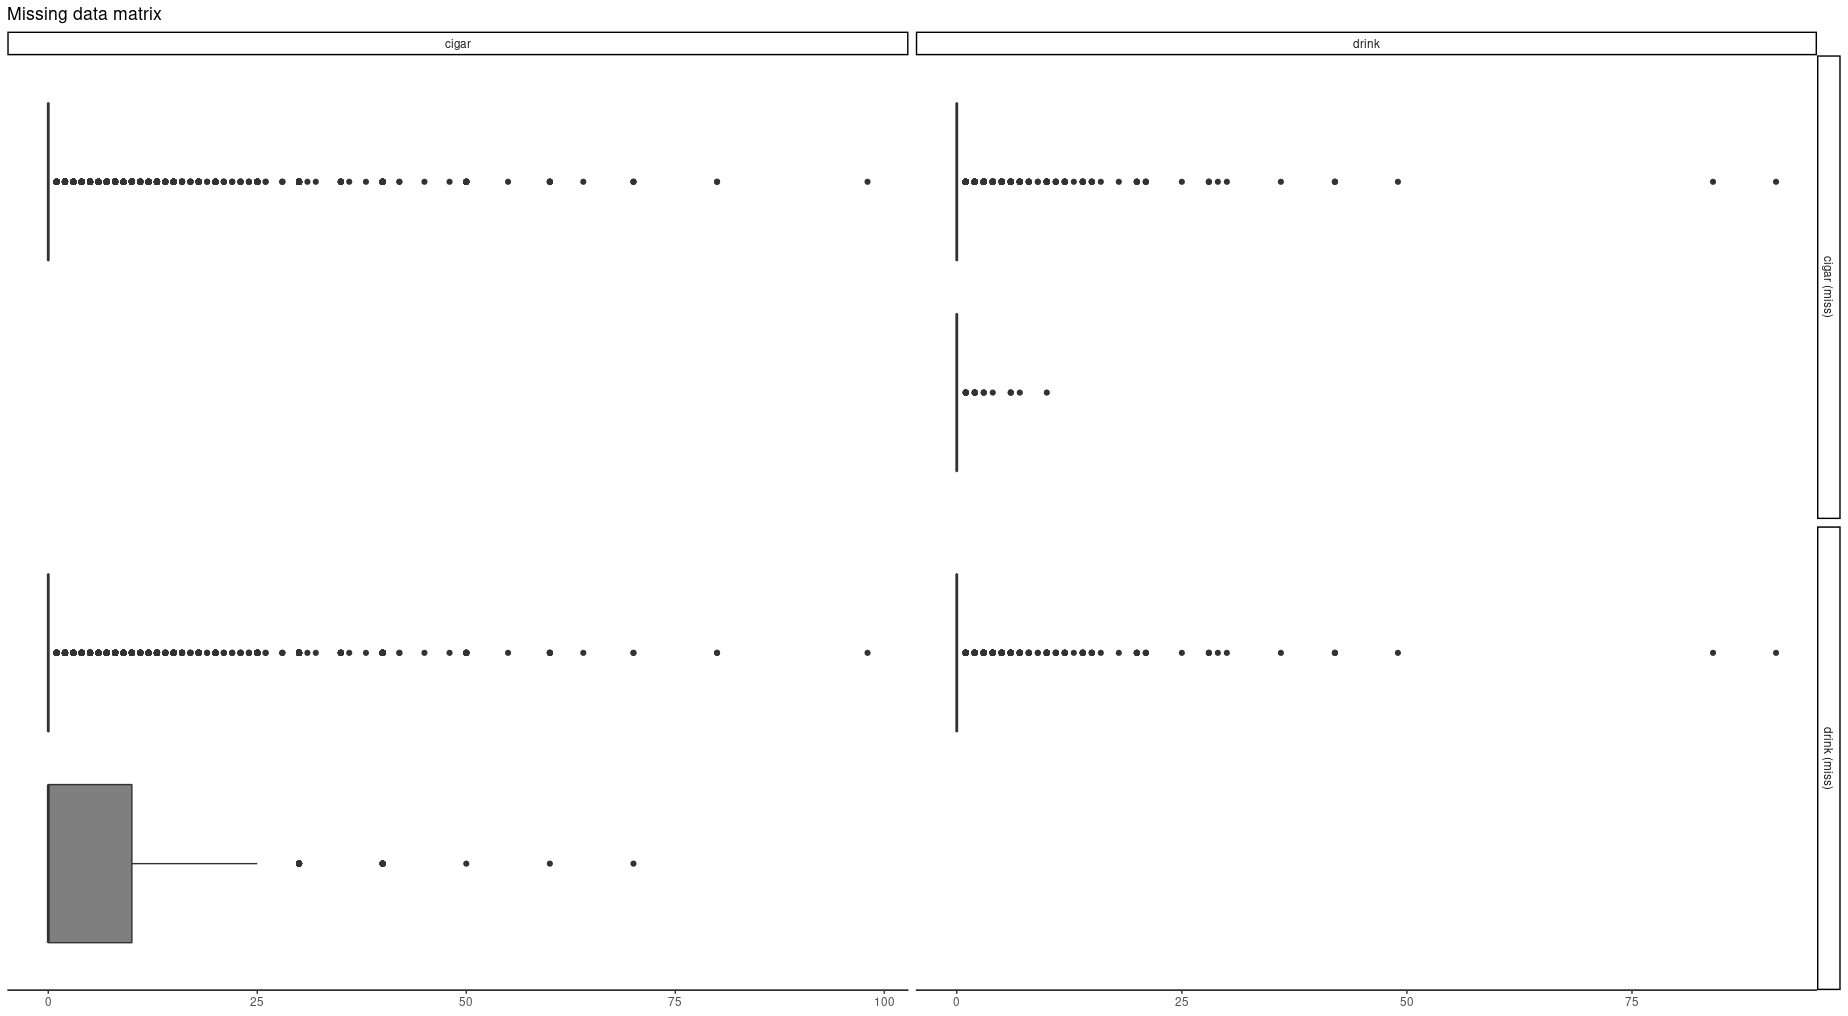
\includegraphics[width=0.7\textwidth]{2b-missing_plots_cigar-vs-drink.png}
\caption{Looking closer at the missingness relationship between drinking and smoking.}
\label{fig-2b2}
\end{figure}
\FloatBarrier



%%%%%%%%%%%%%%%%%
%     Part c   %
%%%%%%%%%%%%%%%%%
\vem
\problem{}{
    \begin{enumerate}[label=(\alph*)]
    \setcounter{enumi}{2}
        \item Produce a summary table describing the final analysis data set.
    \end{enumerate} 
}


% A table environment cannot be broken across pages. Delete \begin{table}\centering and \end{table}, replace tabular with longtable, move \caption and label to immediately after \begin{longtable}{..}. And add \usepackage{longtable} to the preamble, of course.


% Table created by stargazer v.5.2.2 by Marek Hlavac, Harvard University. E-mail: hlavac at fas.harvard.edu
% Date and time: Mon, Sep 27, 2021 - 09:11:29 PM

\begin{longtable}{@{\extracolsep{5pt}}lccccccc}
\caption{Table 1: Summary Statistics} 
  \label{}  
\\[-1.8ex]\hline 
\hline \\[-1.8ex] 
Statistic & \multicolumn{1}{c}{N} & \multicolumn{1}{c}{Mean} & \multicolumn{1}{c}{St. Dev.} & \multicolumn{1}{c}{Min} & \multicolumn{1}{c}{Pctl(25)} & \multicolumn{1}{c}{Pctl(75)} & \multicolumn{1}{c}{Max} \\ 
\hline \\[-1.8ex] 
rectype & 114,610 & 1.262 & 0.440 & 1 & 1 & 2 & 2 \\ 
pldel3 & 114,610 & 1.018 & 0.133 & 1 & 1 & 1 & 2 \\ 
birattnd & 114,610 & 1.202 & 0.564 & 1 & 1 & 1 & 5 \\ 
cntocpop & 114,610 & 1.443 & 1.137 & 0 & 0 & 2 & 3 \\ 
stresfip & 114,610 & 41.743 & 2.167 & 0 & 42 & 42 & 55 \\ 
dmage & 114,610 & 27.757 & 5.699 & 12 & 24 & 32 & 49 \\ 
ormoth & 114,610 & 0.091 & 0.522 & 0 & 0 & 0 & 5 \\ 
mrace3 & 114,610 & 1.259 & 0.657 & 1 & 1 & 1 & 3 \\ 
dmeduc & 114,610 & 13.211 & 2.272 & 0 & 12 & 16 & 17 \\ 
dmar & 114,610 & 1.251 & 0.434 & 1 & 1 & 2 & 2 \\ 
adequacy & 114,610 & 1.297 & 0.546 & 1 & 1 & 2 & 3 \\ 
nlbnl & 114,610 & 0.967 & 1.148 & 0 & 0 & 1 & 12 \\ 
dlivord & 114,610 & 1.986 & 1.174 & 1 & 1 & 2 & 14 \\ 
dtotord & 114,610 & 2.420 & 1.520 & 1 & 1 & 3 & 24 \\ 
totord9 & 114,610 & 2.407 & 1.458 & 1 & 1 & 3 & 8 \\ 
monpre & 114,610 & 2.502 & 1.326 & 0 & 2 & 3 & 9 \\ 
nprevist & 114,610 & 11.153 & 3.524 & 0 & 9 & 13 & 49 \\ 
disllb & 114,610 & 350.412 & 362.325 & 0 & 31 & 777 & 777 \\ 
isllb10 & 114,610 & 3.321 & 3.188 & 0 & 0 & 6 & 9 \\ 
dfage & 114,610 & 30.062 & 6.410 & 13 & 26 & 34 & 78 \\ 
orfath & 114,610 & 0.095 & 0.531 & 0 & 0 & 0 & 5 \\ 
dfeduc & 114,610 & 13.277 & 2.325 & 0 & 12 & 16 & 17 \\ 
birmon & 114,610 & 6.474 & 3.394 & 1 & 4 & 9 & 12 \\ 
weekday & 114,610 & 4.047 & 1.881 & 1 & 2 & 6 & 7 \\ 
dgestat & 114,610 & 39.153 & 2.445 & 17 & 38 & 40 & 47 \\ 
csex & 114,610 & 1.485 & 0.500 & 1 & 1 & 2 & 2 \\ 
dbrwt & 114,610 & 3,373.291 & 585.175 & 227 & 3,062 & 3,742 & 6,067 \\ 
dplural & 114,610 & 1.028 & 0.174 & 1 & 1 & 1 & 4 \\ 
omaps & 114,610 & 8.117 & 1.260 & 0 & 8 & 9 & 10 \\ 
fmaps & 114,610 & 9.009 & 0.707 & 0 & 9 & 9 & 10 \\ 
clingest & 114,610 & 39.109 & 2.057 & 17 & 38 & 40 & 44 \\ 
delmeth5 & 114,610 & 1.549 & 1.010 & 1 & 1 & 1 & 5 \\ 
anemia & 114,610 & 1.990 & 0.099 & 1 & 2 & 2 & 2 \\ 
cardiac & 114,610 & 1.993 & 0.083 & 1 & 2 & 2 & 2 \\ 
lung & 114,610 & 1.993 & 0.085 & 1 & 2 & 2 & 2 \\ 
diabetes & 114,610 & 1.973 & 0.162 & 1 & 2 & 2 & 2 \\ 
herpes & 114,610 & 1.994 & 0.078 & 1 & 2 & 2 & 2 \\ 
chyper & 114,610 & 1.992 & 0.087 & 1 & 2 & 2 & 2 \\ 
phyper & 114,610 & 1.969 & 0.172 & 1 & 2 & 2 & 2 \\ 
pre4000 & 114,610 & 1.986 & 0.119 & 1 & 2 & 2 & 2 \\ 
preterm & 114,610 & 1.986 & 0.118 & 1 & 2 & 2 & 2 \\ 
tobacco & 114,610 & 1.841 & 0.366 & 1 & 2 & 2 & 2 \\ 
cigar & 114,610 & 1.907 & 5.297 & 0 & 0 & 0 & 98 \\ 
cigar6 & 114,610 & 0.346 & 0.861 & 0 & 0 & 0 & 5 \\ 
alcohol & 114,610 & 1.990 & 0.098 & 1 & 2 & 2 & 2 \\ 
drink & 114,610 & 0.031 & 0.619 & 0 & 0 & 0 & 91 \\ 
drink5 & 114,610 & 0.020 & 0.230 & 0 & 0 & 0 & 4 \\ 
wgain & 114,610 & 30.356 & 11.884 & 0 & 23 & 37 & 98 \\ 
\hline \\[-1.8ex] 
\end{longtable	} 



\newpage
%%%%%%%%%%%%%%%%%%%%%%%%%%%%%%%%%%%%%%%%%%%%%%%
%                Problem 3                    %
%%%%%%%%%%%%%%%%%%%%%%%%%%%%%%%%%%%%%%%%%%%%%%%
\problem{3. Smoking and birth weight}{
The next part of the assignment is to try to estimate the “causal” effect of maternal
smoking during pregnancy on infant birth weight. Let’s start out using techniques that
are familiar, and think about whether they are likely to work in this context. Answer
the following questions.\\

    \begin{enumerate}[label=(\alph*)]
    \item Compute the mean difference in APGAR scores (both five and one minute versions) as well as birthweight by smoking status.
    \end{enumerate} 
}

Denote the group with tobacco usage during pregnancy as group 1, and without tobacco usage as group 2. On average, group 2 has 0.043 and 0.013 higher APGAR scores on one and five minute versions respectively. A simple t-test demonstrates they are significant at 1 and 5\% significance levels, respectively. Furthermore, group 2 has average birth-weight 246 grams higher, significant at 1\% significance level.

\begin{table}[ht]
\centering
\begin{tabular}{rrrrrrrrrll}
  \hline
 & Mean\_Smoker & Mean\_NonSmoker & Diff\_Means & statistic & p.value & 95\% conf.int \\ 
  \hline
1m APGAR & 8.072 & 8.115 & -0.043 & -4.300 & 0.000 & [-0.062, -0.024] \\ 
5m APGAR & 8.992 & 9.005 & -0.013 & -2.311 & 0.023 & [-0.024, -0.002] \\ 
BWHT & 3160.306 & 3407.223 & -246.917 & -55.214 & 0.000 & [-255.683, -238.152] \\ 
   \hline
\end{tabular}
\end{table}

%%%%%%%%%%%%%%%%%
%     Part b    %
%%%%%%%%%%%%%%%%%
\vem
\problem{}{
    \begin{enumerate}[label=(\alph*)]
    \setcounter{enumi}{1}
    \item Under what circumstances can one identify the average treatment effect of maternal smoking by comparing the unadjusted difference in mean birth weight of infants of smoking and non-smoking mothers? Estimate its impact under this assumption. Provide and comment on some evidence for or against the validity of the assumption (A useful “Table 1” of any paper is one that describes the overall averages of the observations, and then describes the subsets of people who do and do not receive the treatment (when it is binary)).
    \end{enumerate} 
}

If assignment of maternal smoking was completely random, the differences in means that was reported in Q3-Part(a) would be the ATE of maternal smoking on infant birth-weight. Then, just as in any RCTs, we would see balance across two-groups on any observable variables measured before the 'hypothetical assignment' of maternal smoking. Assume treatment of smoking during pregnancy were assigned in the very early stages of pregnancy, then we must observe balance across the 'treatment' and 'control' groups of covariates either fixed (e.g. age, race) or measured before pregnancy (e.g. chronic conditions), which we deemed amounts to 15 variables in the data-set. However, the balance table below suggests that balance is generally not reached across 9 of 15 covariates based on indicator variable for maternal smoking, which clearly indicates non-random smoking patterns.

\begin{figure}[h!tp]
    \centering
    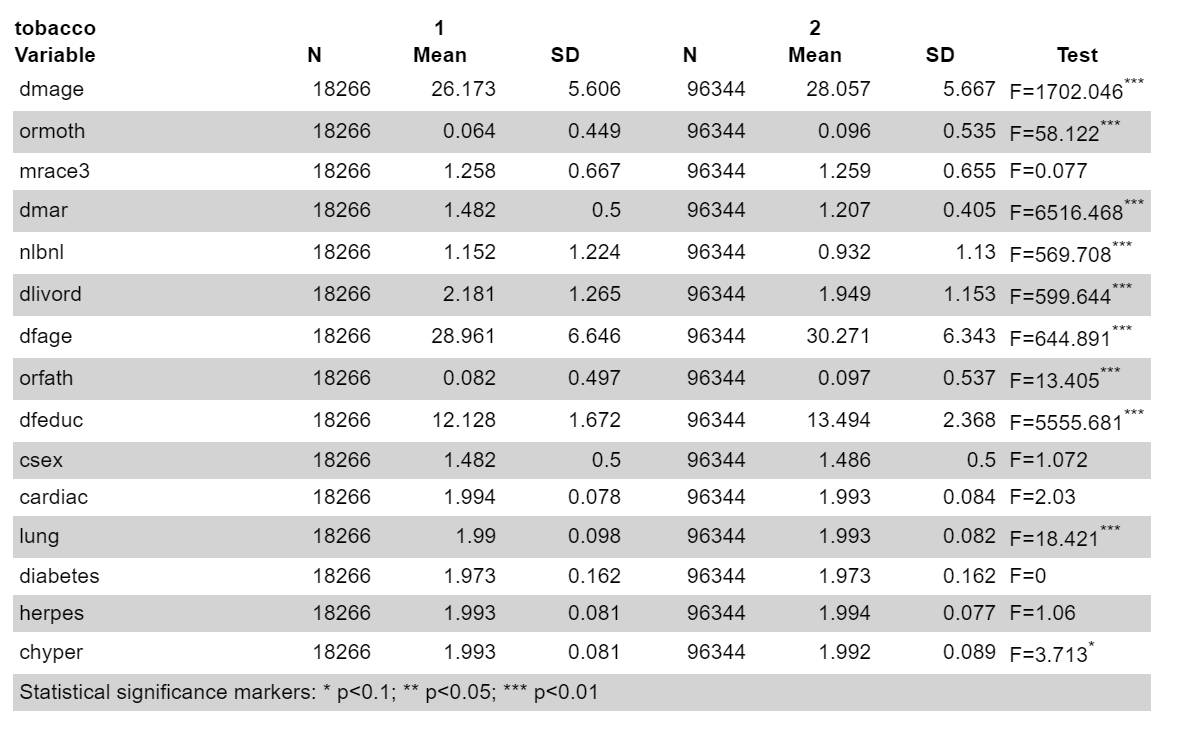
\includegraphics[width=18cm]{3b_BalanceTable_R.png}
\end{figure}

%%%%%%%%%%%%%%%%%
%     Part c    %
%%%%%%%%%%%%%%%%%
\vem
\problem{}{
    \begin{enumerate}[label=(\alph*)]
    \setcounter{enumi}{2}
        \item Suppose that maternal smoking is randomly assigned conditional on the  other observable “predetermined” determinants of infant birth weight. First discuss which (if any) of the variables contained in the data set can clearly be considered to be predetermined. In general, what kinds of variables can be considered predetermined and what kinds of variables cannot?
    \end{enumerate} 
}

Generally, predetermined variables are those which are determined prior to the treatment period--in this case, prior to the decision to smoke. These are most obviously ascriptive characteristics such as race and sex, but could also variables that are clearly uncorrelated with treatment. In our case, these would be race (mrace3), sex (csex), heart condition (cardiac), diabetes (diabetes), herpes (herpes), and hypertention (chyper). 

The variable that most obviously cannot be considered "predetermined" is lung issues (lung) since smoking has been proven to directly cause lung issues. Other variables like education (dfeduc) are somewhere in between predetermined and not.

When running a regression, it is particularly important to control for the variables that are correlated with both treatment and birth weight if we want to isolate the causal impact of smoking on birth weight.

%%%%%%%%%%%%%%%%%
%     Part d    %
%%%%%%%%%%%%%%%%%
\vem
\problem{}{
    \begin{enumerate}[label=(\alph*)]
    \setcounter{enumi}{3}
        \item What does ``selection on observables'' imply about the relationship between maternal smoking and unobservable determinants of birth weight conditional on the observables? Use a basic linear regression model, in conjunction with your answer to part (c), to estimate the impact of smoking and report your estimates. Under what circumstances is the average treatment effect identified?
    \end{enumerate} 
}
Selection on observables implies that maternal smoking is conditionally independent of unobserved factors (conditional on the $X$'s we have observed).

If the covariates we included in our regression include all possible (relevant) covariates that are correlated with both smoking and birth weight and if the covariates of the mothers across all smoking categories share the same support, then the relationship from a regression of birth weight on smoking status will give us the true ATE  of smoking on baby weight. 

Below regressions suggest that smoking decreases birthweight by approximately 218 grams with statistical significance at 1\% significance; smoking increases 1 minute and 5 minute APGAR scores, but this is statistically insignificant at all usual signifiance levels.

\begin{table}[!htbp] \centering 
  \caption{Linear Regression Selection on Observables} 
\begin{tabular}{@{\extracolsep{5pt}}lD{.}{.}{-3} D{.}{.}{-3} D{.}{.}{-3} } 
\\[-1.8ex]\hline 
\hline \\[-1.8ex] 
 & \multicolumn{3}{c}{\textit{Dependent variable:}} \\ 
\cline{2-4} 
\\[-1.8ex] & \multicolumn{1}{c}{dbrwt} & \multicolumn{1}{c}{omaps} & \multicolumn{1}{c}{fmaps} \\ 
\\[-1.8ex] & \multicolumn{1}{c}{(1)} & \multicolumn{1}{c}{(2)} & \multicolumn{1}{c}{(3)}\\ 
\hline \\[-1.8ex] 
 tobacco & 217.986^{***} & -0.011 & -0.010 \\ 
  & (4.753) & (0.011) & (0.006) \\ 
  & & & \\ 
 rectype & -47.944^{***} & -0.044^{***} & -0.016^{***} \\ 
  & (3.867) & (0.009) & (0.005) \\ 
  & & & \\ 
 pldel3 & 142.614^{***} & 0.182^{***} & 0.208^{***} \\ 
  & (14.231) & (0.032) & (0.018) \\ 
  & & & \\ 
 dmage & -4.559^{***} & -0.007^{***} & -0.003^{***} \\ 
  & (0.527) & (0.001) & (0.001) \\ 
  & & & \\ 
 ormoth & -31.493^{***} & -0.032^{***} & -0.019^{***} \\ 
  & (4.153) & (0.009) & (0.005) \\ 
  & & & \\ 
 mrace3 & -105.103^{***} & -0.074^{***} & -0.046^{***} \\ 
  & (2.929) & (0.007) & (0.004) \\ 
  & & & \\ 
 delmeth5 & -10.360^{***} & -0.098^{***} & -0.032^{***} \\ 
  & (1.643) & (0.004) & (0.002) \\ 
  & & & \\ 
 diabetes & -65.834^{***} & 0.165^{***} & 0.067^{***} \\ 
  & (10.190) & (0.023) & (0.013) \\ 
  & & & \\ 
 chyper & 264.745^{***} & 0.266^{***} & 0.144^{***} \\ 
  & (18.750) & (0.042) & (0.024) \\ 
  & & & \\ 
 21 other covariates &  &  &  \\ 
  not shown & & & \\   
  & & & \\   
 Constant & 1,558.841^{***} & 6.942^{***} & 8.099^{***} \\ 
  & (88.273) & (0.199) & (0.112) \\ 
  & & & \\ 
\hline \\[-1.8ex] 
Observations & \multicolumn{1}{c}{114,610} & \multicolumn{1}{c}{114,610} & \multicolumn{1}{c}{114,610} \\ 
R$^{2}$ & \multicolumn{1}{c}{0.109} & \multicolumn{1}{c}{0.021} & \multicolumn{1}{c}{0.024} \\ 
Adjusted R$^{2}$ & \multicolumn{1}{c}{0.109} & \multicolumn{1}{c}{0.021} & \multicolumn{1}{c}{0.024} \\ 
Residual Std. Error (df = 114579) & \multicolumn{1}{c}{552.347} & \multicolumn{1}{c}{1.246} & \multicolumn{1}{c}{0.699} \\ 
F Statistic (df = 30; 114579) & \multicolumn{1}{c}{468.596$^{***}$} & \multicolumn{1}{c}{81.881$^{***}$} & \multicolumn{1}{c}{93.051$^{***}$} \\ 
\hline 
\hline \\[-1.8ex] 
 & \multicolumn{3}{r}{$^{*}$p$<$0.1; $^{**}$p$<$0.05; $^{***}$p$<$0.01} \\ 
\end{tabular} 
\end{table}



%%%%%%%%%%%%%%%%%%%%%%%%%%%%%%%%%%%%%%%%%%
%            R CODE 
%%%%%%%%%%%%%%%%%%%%%%%%%%%%%%%%%%%%%%%%%%
\newpage
\section*{The Code}
\begin{lstlisting}[language=R]

## ---------------------------
## R version 3.6.3 (2020-02-29)
## Script name: ps1a.R
##
## Purpose of script: run code necessary for ps1a fro ARE 213
## Date Created: 2021-09-27
##
## ---------------------------


## PACKAGES ===========================================
# install.packages("pacman")
# install.packages("plm")
install.packages('foreign')
install.packages('stargazer')
install.packages("finalfit")
library(tidyverse)
library(foreign)
library(xtable)
library(stargazer)
library(finalfit) 


## PROBLEM 1 =========================================
N = c(40046, 26107, 256423)
D = c(1263, 98, 1422)
R = c(315, 37, 59)

R = D/N*10^4
za = qnorm(0.025, lower.tail=FALSE)
p = 1/N * D
varR = p*(1-p)/N
R_lower = R - 10^4*za*(varR)^0.5
R_upper= R + 10^4*za*(varR)^0.5

df = data.frame(R=R, CI_lower=R_lower, CI_upper=R_upper)
print(xtable(df, type = "latex"))


## PROBLEM 2 =========================================
data = read.dta('ps1.dta')

## PART (a) . . . . . . . . . . . . . . . . . . . . . 
missing_codes = read.csv('missing_codes.csv')
mvars = as.character(missing_codes$varname)
missing_codes$num_missing = as.integer(0)
for (row in 1:nrow(missing_codes)) {
  var = as.character(missing_codes[row, "varname"])
  code  = as.numeric(missing_codes[row, "missing_code"])
  nmissing = as.integer(sum(data[, var] == code))
  missing_codes$num_missing[missing_codes$varname==var] = nmissing
  data[, var] = na_if(data[, var], code)
}
print(xtable(missing_codes, type = "latex", caption = 'Missing values, by variable name.'), 
      caption.placement = 'top', include.rownames=FALSE)

# Dataframe with missing dropped
df = data[complete.cases(data), ]


## PART (b) . . . . . . . . . . . . . . . . . . . . . 
data %>% ff_glimpse()
data %>% missing_plot()
data %>% missing_pattern()

for (var in colnames(data)) {
  print('*********************************')
  print(var)
  print(sort(unique(data[, var])))
}

# Convert all variables with <7 unique values to factor (and 3 additional variables)
factor_vars = c("isllb10", "birmon", "weekday")
for (var in colnames(data)) {
  print('*********************************')
  print(var)
  print(length(unique(data[, var])))
  if (length(unique(data[!is.na(data[, var]), var])) < 7 || var %in% factor_vars) {
    data[, var] = factor(data[, var])
  }
}

data[, mvars] %>% missing_pairs(position = "fill")
explore_vars = c("cigar", "drink")
data[, explore_vars] %>% missing_pairs(position = "fill")
data[, mvars]  %>% missing_compare()


# Create variable "na" if any variable has missing data
df$na <- complete.cases(df)
table(df$na, useNA = "always")

# t Test - Comparison of Means of each variable between two samples
# (Observations with complete data vs Observations with any missing data)
ttest_res <- lapply(names(select(df, -na)), function(x) 
  t.test(as.formula(paste(x, "~", "na")), data = df))

count <- 0
for (i in 1:(length(names(df))-1)) {
  if (ttest_res[[i]]$p.value < 0.05) {
    count <- count + 1
  }
}
count 
# We see support for alternative hypotheses that there is 
# statistical difference between the observations with and without 
# missing observations 37 out of 48 variables at the 95% confidence level.



## PART (c) . . . . . . . . . . . . . . . . . . . . . 
stargazer(df, title="Table 1: Summary Statistics", out="summary_stats_2c.tex")
# For long table (across multiple pages):
# A table environment cannot be broken across pages. 
# Delete \begin{table}\centering and \end{table}, replace tabular with longtable, 
# move \caption and label to immediately after \begin{longtable}{..}. 
# And add \usepackage{longtable} to the preamble, of course.




## PROBLEM 3 =========================================
## PART (a) . . . . . . . . . . . . . . . . . . . . . 
# "dbrwt" = birthweight in grams

#omaps, fmaps, dbrwt, tobacco, cigar, cigar6
test1 <- t.test(omaps~tobacco, data = df)
test2 <- t.test(fmaps~tobacco, data = df)
test3 <- t.test(dbrwt~tobacco, data = df)

tab <- map_df(list(test1, test2, test3), tidy) %>% 
  rename(Differences_In_Means = estimate, Mean_Maternal_Smokers = estimate1, Mean_Maternal_Non_Smokers = estimate2)

print(xtable(tab, type = "latex"), file = "Q3a.tex")


## PART (b) . . . . . . . . . . . . . . . . . . . . . 
df_3b <- select(df_nona, dmage, ormoth, mrace3, dmar, nlbnl, dlivord, dfage, orfath, dfeduc, csex, cardiac, lung, diabetes, herpes, chyper, tobacco)

sumtable(df_3b, group = 'tobacco', group.test = TRUE)
bal.tab(covs = df_nona, treat=tobacco, data = df_nona)




## PART (c) . . . . . . . . . . . . . . . . . . . . . 






## PART (d) . . . . . . . . . . . . . . . . . . . . . 
reg1 <- lm(dbrwt ~ tobacco + rectype + pldel3 + birattnd + cntocpop + stresfip + dmage + 
             ormoth + mrace3 + dmeduc + dmar + adequacy + nlbnl + dlivord + dtotord + 
             totord9 + nprevist + disllb + isllb10 + dfage + orfath + dfeduc + 
             weekday + csex + delmeth5 + cardiac + diabetes + herpes + chyper + 
             preterm, data = df_nona)

reg2 <- lm(omaps ~ tobacco + rectype + pldel3 + birattnd + cntocpop + stresfip + dmage +
             ormoth + mrace3 + dmeduc + dmar + adequacy + nlbnl + dlivord + dtotord + 
             totord9 + nprevist + disllb + isllb10 + dfage + orfath + dfeduc + 
             weekday + csex + delmeth5 + cardiac + diabetes + herpes + chyper + 
             preterm, data = df_nona)

reg3 <- lm(fmaps ~ tobacco + rectype + pldel3 + birattnd + cntocpop + stresfip + dmage + 
             ormoth + mrace3 + dmeduc + dmar + adequacy + nlbnl + dlivord + dtotord + 
             totord9 + nprevist + disllb + isllb10 + dfage + orfath + dfeduc + 
             weekday + csex + delmeth5 + cardiac + diabetes + herpes + chyper + 
             preterm, data = df_nona)

stargazer(reg1, reg2, reg3, title="Linear Regression Selection on Observables", align = TRUE)
\end{lstlisting}



\end{document}

References
